\chapter{Context}

% As of today little work has been done on creating a multihop LoRa Network (see Kris Paper on RPL LoRa in context section)

\section{LoRa}

\label{section:lora}

\paragraph{Packet Format}
\paragraph{Chirp Spread Spectrum (CSS) modulation}
\paragraph{Transmission Power}
\paragraph{Spreading Factor}

The higher the \emph{SF} the longer the communication range get while the
transmission also get slower. Frames can be sent at the same time if they are
all sent with a different spreading factors\cite{8030482}.

The data rate can range from 0.3kbps to 27kbps depending on the \emph{SF} % TODO Calculation needed

\paragraph{Bandwidth}
\paragraph{Coding-Rate}
\paragraph{Channels}

% See 'Understanding the limits of LoRaWAN' the 3 channels definition in Europe

\paragraph{Time On Air}

\begin{equation}
  \label{eq:tsym}
  T_{sym} = \frac{2^{SF}}{BW}
\end{equation}
\begin{equation}
  \label{eq:tpreamble}
  T_{preamble} = (n_{preamble} + 4.25)T_{sym}
\end{equation}
\begin{equation}
  \label{eq:payloadsymnb}
  payloadSymbNb = 8 + \max(ceil(\frac{8PL - 4SF + 28 + 16 - 20H}{4(SF - 2DE)})(CR + 4),0)
\end{equation}
\begin{equation}
  \label{eq:tpayload}
  T_{payload} = payloadSymNb T_{sym}
\end{equation}
\begin{equation}
  \label{eq:tpacket}
  T_{packet} = T_{preamble} + T_{paylaod}
\end{equation}

\section{TSCH}

TSCH is a MAC layer protocols designed for the low power and reliable
communications.
% And aims to achieve that 

\begin{description}
  \item[Channel Hopping] for a better usage of the band and less interference.
  \item[Time-division multiple access] or (TDMA) by assigning time-slots for each
    participant in the network avoiding collisions.
  \item[Synchronization] time-synchronized nodes syncing their clock with each
    other.
\end{description}

In the following section I will present the TSCH building blocks.

\subsection{Time Slots}

Time slots are a fixed unit of time to execute the TSCH network operations. 
The duration of the time slot is not standardized and depend on the physical 
layer we are using. 
Although, it has to be long enough for the longest frame size to be sent
between two nodes with an acknowledgement~\cite{rfc7554}. 
All time slots in a TSCH network have to be the same duration.

For each time slots operations, a schedule orchestrate what each
node of the network will use his time-slot for.

\begin{description}
  \item [Transmit] if a packet is on the outgoing buffer of the node.
  \item [Receive] listen for incoming packets that may arrive.
  \item [Sleep]
\end{description}

Because \emph{Channel Hopping} increase the network capacity a single time-slot
can be shared between multiple device to transmit at the same time on different
channels.

We can define \emph{links} as being made up of time slots and
channels~\cite{Chen2013PerformanceAO}.

\begin{equation}
  \label{eq:links}
  link = (TimeSlot_{number}, Channel_{offset})
\end{equation}

Multiple links constitute a time slot (dependent on the number of channel
available). Devices can transmit on different links during the same time slot.

\subsection{Slotframes}

Slotframes are a group of time slots that repeats over time as represented
in~\ref{fig:timeslots}. 

The size of the slotframe will directly impact on the energy consumption of
each node as increasing the size will decrease the number of time a node has
to exit sleep mode to listen or transmit packets.

\begin{figure}[H]
  \centering

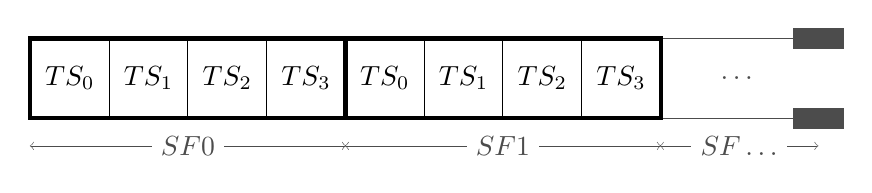
\begin{tikzpicture}[
  timeslot/.style={draw, rectangle, minimum size=1cm},
  arr/.style={help lines,black!70,<->},
]

\foreach [evaluate={\ts=int(mod(\i, 4))}] \i in {0,...,7} {
  \node (ts\i) [timeslot] at (\i, 0) {$TS_{\ts}$};
}
\node (ts8) [minimum height=1cm, minimum width=2cm, black!70] at (8.5, 0) {\ldots};
\draw[help lines, black!70]
  (ts8.north west) -- (ts8.north east) node[fill=white, black!70] {$\ldots$};
\draw[help lines, black!70]
  (ts8.south west) -- (ts8.south east) node[fill=white, black!70] {$\ldots$};

\draw[ultra thick] 
  (ts0.south west) rectangle (ts3.north east)
  (ts4.south west) rectangle (ts7.north east);

\draw[arr]
  ([yshift=-10pt]ts0.south west) -- node[fill=white] {$SF0$} ([yshift=-10pt]{ts3.south east});
\draw[arr]
  ([yshift=-10pt]ts4.south west) -- node[fill=white] {$SF1$} ([yshift=-10pt]{ts7.south east});
\draw[arr]
  ([yshift=-10pt]ts8.south west) -- node[fill=white] {$SF\ldots$} ([yshift=-10pt]{ts8.south east});

\end{tikzpicture}

\caption{Slotframes representation\label{fig:timeslots}}
\end{figure}


\subsection{Scheduling}

\subsection{Absolute Slot Number}

ASN is a shared counter between all the devices that define the number of time slots 
elapsed since the start of the start of the network.
It is increased after each time slot.

\subsection{Channel Hopping}

\subsection{Synchronization}

\paragraph{Cost of the Synchronization}

% * Nodes are required to synchronize their time source periodically
% * It's highly dependant on the clock quality

\section{6LoWPAN}

% 6TOP Sublayer

\section{Contiki OS}

\section{Related work}

\subsection{Time-Slotted LoRa}

\subsection{Multihop LoRa}


